\documentclass[12pt,a4paper]{report}
\usepackage[margin=1in]{geometry}
\usepackage{graphicx}
\usepackage{amsmath, amssymb, amsthm}
\usepackage{souce}
\usepackage{setspace}
\usepackage{enumitem}
\usepackage{booktabs,longtable,threeparttable,siunitx,tabularx,makecell}
\usepackage{xcolor, listings}

% Python listings settings
\lstset{,
	basicstyle      = \ttfamily\small,
	language        = Python,            
	breaklines       = true,
	keywordstyle     = \color{blue},
	commentstyle     = \color{green!60!black},
	identifierstyle  = \color{black},
	stringstyle      = \color{orange},
	showstringspaces = false,
	stepnumber       = 1,
	numbersep        = 5pt,
	frame            = single,
	tabsize          = 4,
	captionpos       = b,
	morekeywords     = {import, def, return, for, in, if, else, np, linalg, time}
}


\graphicspath{{figures/}}

\usepackage{etoolbox}
\makeatletter
\patchcmd{\chapter}{\clearpage}{}{}{}
\makeatother

\usepackage{pdfpages}
\usepackage{pdflscape,rotating}
\usepackage{adjustbox}

\usepackage[style=apa, backend=biber]{biblatex}
\usepackage{csquotes}
\addbibresource{reference.bib}
\usepackage[hidelinks]{hyperref}
\usepackage{url}

\newtheorem{definition}{Definition}[chapter]
\newtheorem{theorem}{Theorem}[chapter]

\usepackage{float}
\usepackage{ragged2e}
\author{
Franniel Luigi Hilario
}


\begin{document}
\emergencystretch 3em
\sloppy
\onehalfspacing

\begin{titlepage}
\pagenumbering{gobble}
\centering % Set the line spacing to 1 for the title page.

\begin{minipage}[c][3\baselineskip][c]{0.9\linewidth}
\centering\bfseries\large\MakeUppercase{
On the Performance of Linear System Solvers in Alternating Least Squares for Collaborative Filtering
}
\end{minipage}

\vspace{0.5in}
{\centering Franniel Luigi Hilario \quad Brian Gabriel Magbanua  \quad Fiona Ventura\\ Jermaine Pasamba \quad Mark Oliver Medina  }

\vspace{0.5in}

{
College of Science, Bachelor of Science in Mathematics
With Specialization in Computer Science,
Bulacan State University, Malolos, Bulacan
}

\vspace{1in}
\begin{abstract}
\begin{justify}
This study evaluates the impact of linear system solvers on the performance of Alternating Least Squares (ALS) for collaborative filtering using the MovieLens 100K dataset. Five solver within the ALS update step was analyzed such as, explicit matrix inversion, Gaussian elimination with partial pivoting, LU decomposition, QR decomposition, and Cholesky decomposition. Under a fixed experimental setup ($K=10$, $\lambda=10$, and 30 epochs), the investigation examines computational efficiency, numerical stability, and recommendation quality. Results indicate that recommendation quality, measured by train and test RMSE trajectories, remains effectively identical across all correctly implemented solvers, suggesting that solver choice does not materially affect prediction accuracy on this benchmark. However, significant differences emerge in runtime and numerical precision. Cholesky decomposition, by exploiting the symmetric positive definite structure of the ALS subproblem, provides the most efficient and numerically stable solution. Conversely, explicit matrix inversion exhibits the highest computational cost and largest residual norms $\|Ax-b\|$. The findings support selecting solvers primarily based on computational efficiency for well-conditioned ALS subproblems, while emphasizing the use of robust factorization methods in more demanding numerical settings. This research demonstrates that while solver selection does not impact the final recommendation output, it is a critical engineering decision for optimizing the speed and stability of recommender system training.
\end{justify}
\end{abstract}
\end{titlepage}
\pagenumbering{arabic}
\chapter*{Introduction}

Recommender systems have become an essential component of modern information platforms which assist users to find relevant content in environments that contain extensive item collections and users who have restricted viewing time. The system uses past user behavior data to identify user preferences which it uses to generate customized content suggestions for e-commerce platforms and streaming services and social media networks \parencite{ricci2015recommender}. Collaborative filtering stands out among recommendation methods because it can successfully identify user preferences based on user-item interaction patterns which it derives from data analysis without needing direct item attribute knowledge \parencite{koren2009matrix}.

The Netflix Prize competition created a key development for collaborative filtering by pushing researchers to build recommendation systems which could handle large datasets while providing precise predictions. Matrix factorization emerged as the leading framework from this era because it uses a user-item rating matrix which requires two low-rank latent factor matrices to create user preference and item characteristic representations \parencite{koren2009matrix,takacs2009scalable}. The system uses this formulation to reveal hidden patterns between users and items while handling computational demands of extensive datasets.

The matrix factorization computation field has made Alternating Least Squares (ALS) into a common method because of its basic operation design which delivers strong results and works well with parallel processing. The ALS method breaks down its optimization task into two parts which need to change user and item latent factor matrices. The algorithm needs numerical linear algebra routines to deliver both computational efficiency and stability because the update process needs to solve multiple regularized least-squares problems \parencite{zhou2008large}.

The existing body of research on recommender systems has received extensive coverage, yet most investigations concentrate on developing model architectures and implementing regularization techniques and building feature engineering systems. The numerical methods which apply to ALS least-squares subproblem resolution have received less research attention when compared to model architecture and regularization methods and feature engineering systems. Subproblems can use multiple linear algebra methods for solving which include explicit matrix inversion and direct factorization methods and iterative solvers.

The numerical linear algebra field treats these two options as different solutions. The traditional results demonstrate that explicit matrix inversion method operates at lower numerical stability which decreases its efficiency compared to linear system solving through factorization methods which include QR or Cholesky decomposition \parencite{trefethen1997numerical, golub2013matrix}. The solver selection process affects both computational speed and the ability to reach a solution while maintaining system stability.

Small-to-medium benchmark datasets such as the MovieLens 100K dataset create a perfect testing ground to study these performance differences. The dataset enables controlled research which shows how solver selection affects outcomes because it is widely used and requires low computational power while all model components remain unchanged. The study of solver-level operations at this location delivers important findings which help both educational functions and actual implementations of recommender system operations.

\section{Objectives}
The main goal of this research is to analyze the performance of different linear system solvers in the context of Alternating Least Squares (ALS) for collaborative filtering. The specific objectives include:
\begin{enumerate}
\item Compare the computational efficiency of the following linear system solvers for solving the least-squares subproblems in ALS:
\begin{enumerate}[label*=\arabic*.]
\item Explicit Matrix inversion,
\item Partial pivoting,
\item LU decomposition,
\item QR decomposition, and
\item Cholesky decomposition
\end{enumerate}
\item Evaluate the numerical stability of each solver by analyzing the condition number of the matrices involved and the sensitivity of the solutions to perturbations in the input data.
\item Assess the impact of solver choice on the overall performance of the ALS algorithm in terms of convergence speed and the quality of the recommendations generated.

\end{enumerate}

\vspace{4em}

\chapter*{Preliminaries}

The necessary mathematical background for understanding the performance of linear system solvers in Alternating Least Squares (ALS) for collaborative filtering includes matrix factorization and numerical linear algebra techniques.

\section{Collaborative Filtering and Matrix Factorization}

Every day, millions of people receive personalized recommendations from movies on Netflix to products on Amazon without ever having to explicitly describe what they like. Behind many of these systems lies a simple but powerful idea: \textit{people who agreed in the past are likely to agree in the future}. If two users have rated the same set of movies similarly, it is reasonable to assume that they share similar tastes, and that a movie one of them enjoyed might appeal to the other as well. This principle is the foundation of \textbf{collaborative filtering} \parencite{ricci2015recommender}.

Collaborative filtering works purely from observed user behavior such as ratings, clicks, and purchases without needing to know anything about the items themselves. A streaming platform does not need to know that a film is a thriller or that it stars a particular actor; it only needs to know who watched it and how they rated it.

\subsection*{The Rating Matrix}

The starting point for collaborative filtering is the \textbf{user-item rating matrix}. Imagine a large table where each row represents a user and each column represents an item. The entry at row \( i \) and column \( j \), denoted \( R_{ij} \), is the rating that user \( i \) gave to item \( j \). The goal of a recommender system is to fill in the missing entries of this table to predict how a user would rate items they have not yet seen.

This matrix \( R \in \mathbb{R}^{m \times n} \) is extremely sparse (mostly zeroes) with millions of users and items, the vast majority of entries are unobserved. A typical user rates only a tiny fraction of all available items, which makes the prediction problem challenging.

\subsection*{Matrix Factorization}

One of the most effective approaches to this problem is \textbf{matrix factorization}. The intuition is that user preferences and item characteristics can be described by some underlying \textit{latent factors}, hidden concepts such as genre, tone, or style that are not explicitly labeled but can be inferred from rating patterns. For instance, a user who consistently rates action movies highly implicitly reveals something about their taste, even if that preference is never explicitly stated.

\begin{definition}[Matrix Factorization]
Matrix factorization approximates the rating matrix \( R \) as the product of two smaller matrices:
\[
R \approx UV^\top
\]
where \( U \in \mathbb{R}^{m \times f} \) is the \textbf{user factor matrix}, \( V \in \mathbb{R}^{n \times f} \) is the \textbf{item factor matrix}, and \( f < \min(m, n) \) is the number of latent factors.
\end{definition}

Each row \( U_i \in \mathbb{R}^f \) is a compact numerical representation of user \( i \)'s preferences, and each row \( V_j \in \mathbb{R}^f \) captures the latent characteristics of item \( j \). The predicted rating for user \( i \) on item \( j \) is the dot product:
\[
\hat{R}_{ij} = U_i^\top V_j
\]

It follows, if both the user vector and the item vector point in the same direction in the latent space, meaning the user tends to like what the item offers, the dot product will be large, indicating a strong predicted preference.

\subsection*{Learning the Factors}

To find the best \( U \) and \( V \), minimizing the difference between the predicted and actual ratings on all observed entries was done. A regularization term is added to prevent overfitting, which is the tendency of a model to memorize training data rather than learning generalizable patterns. This leads to the following objective function:

\[
\mathcal{L}(U, V) = \sum_{(i,j) \in \Omega} \left( R_{ij} - U_i^\top V_j
\right)^2 + \lambda \left( \|U\|_F^2 + \|V\|_F^2 \right)
\]

Where \( \Omega \) is the set of observed ratings, \( \lambda > 0 \) is the regularization parameter that controls how strongly large factor values are penalized, and \( \| \cdot \|_F \) is the Frobenius norm, which measures the overall magnitude of a matrix. The task of the ALS algorithm described in the next section is to minimize this objective efficiently \parencite{koren2009matrix}.

\section{Alternating Least Squares}

Finding \( U \) and \( V \) that simultaneously minimize \( \mathcal{L}(U, V) \) is difficult because the two unknowns are multiplied together, making the problem non-convex. However, there is creative solution, if we temporarily fix one matrix and only optimize the other, the problem simplifies dramatically into a standard least-squares problem, which has a clean closed-form solution. Alternating Least Squares (ALS) does exactly this by repeatedly alternates between optimizing \( U \) with \( V \) held fixed, and optimizing \( V \) with \( U \) held fixed, until the solution converges \parencite{zhou2008large}.

Think of it like adjusting two knobs on a stereo: instead of turning both at once, you fine-tune one while holding the other steady, then switch. Each individual adjustment is straightforward, and repeating this process gradually brings both knobs to their optimal positions.

\subsection*{User Factor Update}

With \( V \) fixed, the problem of finding the best \( U_i \) for each user \( i \) becomes independent for each user, and reduces to minimizing:
\[
    \mathcal{L}(U_i) = \sum_{j \in \Omega_i} \left( R_{ij} - U_i^\top V_j \right)^2
    + \lambda \|U_i\|^2
\]
where \( \Omega_i \) is the set of items that user \( i \) has rated. Setting the derivative of this expression to zero and solving gives the closed-form update:
\[
    \left( V_{\Omega_i}^\top V_{\Omega_i} + \lambda I \right) U_i =
    V_{\Omega_i}^\top R_{i,\Omega_i}
\]
This is a system of linear equations of the form \( Ax = b \), where \( A = V_{\Omega_i}^\top V_{\Omega_i} + \lambda I \) and \( b = V_{\Omega_i}^\top R_{i,\Omega_i} \). Solving it yields the updated latent factor vector for user \( i \).

\subsection*{Item Factor Update}

Similarly, fixing \( U \) and optimizing for each item \( j \) leads to an identical structure:
\[
    \left( U_{\Omega_j}^\top U_{\Omega_j} + \lambda I \right) V_j =
    U_{\Omega_j}^\top R_{\Omega_j,j}
\]
where \( \Omega_j \) is the set of users who have rated item \( j \). Again, this is a linear system \( Ax = b \) of the same form.

\subsection*{The Linear System under ALS}

Both update steps reduce to solving a linear system:
\[
    Ax = b, \quad A = W^\top W + \lambda I \in \mathbb{R}^{f \times f}
\]
where \( W \) is the relevant submatrix of either \( U \) or \( V \). This system is small, the matrix \( A \) is only \( f \times f \), where \( f \) is typically between 10 and 100, but it must be solved once for every user and once for every item at every iteration of ALS. With millions of users and items, this adds up quickly, making the efficiency of the chosen solver a significant factor in the overall runtime of the algorithm \parencite{takacs2009scalable}.

An important property of \( A \) is that it is always \textbf{symmetric positive definite} for any \( \lambda > 0 \). Symmetry means \( A^\top = A \), and positive definiteness means that \( x^\top Ax > 0 \) for all nonzero vectors \( x \), the matrix does not ``collapse'' any direction in space. This guarantees that the linear system has a unique solution at every step, and it also allows certain solvers, particularly Cholesky decomposition, to exploit this structure for improved speed and stability. The full ALS procedure is summarized in Algorithm~\ref{alg:als}.

\begin{figure}[H]
\caption{The ALS algorithm for matrix factorization.}
\label{alg:als}
\centering
\begin{minipage}{0.85\textwidth}
\begin{enumerate}[label=\textbf{Step \arabic*.}]
    \item \textbf{Initialize} \( U \) and \( V \) with small random values.
    \item \textbf{Fix \( V \)}, solve for each row \( U_i \) by solving
          \( \left(V_{\Omega_i}^\top V_{\Omega_i} + \lambda I\right) U_i =
          V_{\Omega_i}^\top R_{i,\Omega_i} \).
    \item \textbf{Fix \( U \)}, solve for each row \( V_j \) by solving
          \( \left(U_{\Omega_j}^\top U_{\Omega_j} + \lambda I\right) V_j =
          U_{\Omega_j}^\top R_{\Omega_j,j} \).
    \item \textbf{Repeat} Steps 2--3 until the change in \( \mathcal{L} \)
          falls below a threshold or a maximum number of iterations is reached.
\end{enumerate}
\end{minipage}
\end{figure}


\section{System of Linear Equation Solvers}

This section presents the five linear system solvers evaluated in this study. Each solver addresses the system \( Ax = b \) where \( A \in \mathbb{R}^{f \times f} \)is the ALS subproblem matrix described above.

\subsection{Explicit Matrix Inversion}

The most straightforward approach is to compute \( A^{-1} \) explicitly and obtain the solution as:
\[
    x = A^{-1} b
\]

\begin{definition}[Matrix Inverse]
    For a nonsingular matrix \( A \in \mathbb{R}^{n \times n} \), the inverse \( A^{-1} \) is the unique matrix satisfying \( A A^{-1} = A^{-1} A = I \).
\end{definition}

The inverse can be computed using the adjugate formula:
\[
    A^{-1} = \frac{1}{\det(A)} \text{adj}(A)
\]
or more practically via row reduction of \( [A \mid I] \). Computing \( A^{-1} \) requires\( \mathcal{O}(n^3) \) operations. While conceptually simple, explicit inversion accumulates rounding errors more aggressively than factorization-based methods, as each element of \( A^{-1} \) is formed from sums and products of all matrix entries \parencite{anton2014elementary}.

\subsection{LU Decomposition}

LU decomposition factors \( A \) into the product of a lower triangular matrix
\( L \) and an upper triangular matrix \( U \):
\[
    A = LU
\]

\begin{definition}[LU Decomposition]
    Given \( A \in \mathbb{R}^{n \times n} \), LU decomposition finds
    \( L, U \in \mathbb{R}^{n \times n} \) where \( L \) is unit lower triangular
    (diagonal entries equal to 1) and \( U \) is upper triangular, such that
    \( A = LU \).
\end{definition}

The system \( Ax = b \) is then solved in two triangular stages:
\begin{align*}
    Ly &= b \quad \text{(forward substitution)} \\
    Ux &= y \quad \text{(back substitution)}
\end{align*}
Each triangular solve costs \( \mathcal{O}(n^2) \), and the factorization itself costs \( \mathcal{O}(n^3) \). The advantage of LU decomposition over explicit inversion is that the triangular structure is exploited directly, reducing numerical error propagation \parencite{anton2014elementary}.

\subsection{Gaussian Elimination with Partial Pivoting}

Gaussian elimination is a systematic method for solving a linear system \( Ax = b \) by reducing the augmented matrix \( [A \mid b] \) to upper triangular form through a sequence of row operations, after which the solution is recovered by back substitution. While straightforward in theory, a naive implementation can fail or produce highly inaccurate results when a pivot element, the leading entry used to eliminate entries below it, is zero or very small, causing division by a near-zero number and amplifying numerical errors. Partial pivoting addresses this by introducing a row-swapping strategy: before each elimination step, the algorithm scans the current column for the entry with the largest absolute value and swaps that row to the pivot position. This ensures that the largest available value is always used as the pivot, keeping the multipliers used during elimination bounded and preventing error amplification \parencite{anton2014elementary}.

\begin{definition}[Gaussian Elimination with Partial Pivoting]
    At the \( k \)-th elimination step, partial pivoting selects the row 
    \( r \geq k \) with the largest absolute value in column \( k \):
    \[
        r = \arg\max_{k \leq i \leq n} |A_{ik}|
    \]
    and swaps row \( r \) with row \( k \) before performing elimination. This 
    is equivalent to factoring a row-permuted version of \( A \):
    \[
        PA = LU
    \]
    where \( P \) is a permutation matrix recording all row swaps, \( L \) is unit lower triangular, and \( U \) is upper triangular.
\end{definition}

The system \( Ax = b \) is then solved in two stages using the factored form:
\begin{align*}
    Ly &= Pb \quad \text{(forward substitution)} \\
    Ux &= y  \quad \text{(back substitution)}
\end{align*}

The overall computational cost is \( \mathcal{O}(n^3) \) for the elimination phase, plus \( \mathcal{O}(n^2) \) for each triangular solve. Gaussian elimination with partial pivoting is the standard general-purpose method for solving dense linear systems and is the default approach in most numerical libraries precisely because it is robust across a wide range of matrix types without requiring any special structure \parencite{anton2014elementary}.

\subsection{Cholesky Decomposition}

When \( A \) is symmetric positive definite, as is the case for ALS subproblem matrices, Cholesky decomposition provides a more efficient and numerically stable factorization:
\[
    A = LL^\top
\]
where \( L \) is a unique lower triangular matrix with positive diagonal entries.

\begin{theorem}[Cholesky Decomposition]
    Every symmetric positive definite matrix \( A \in \mathbb{R}^{n \times n} \)has a unique factorization \( A = LL^\top \) where \( L \) is lower triangular with positive diagonal entries.
\end{theorem}

The diagonal entries of \( L \) and the off-diagonal entries are computed
column by column:
\[
    L_{kk} = \sqrt{A_{kk} - \sum_{j=1}^{k-1} L_{kj}^2}, \qquad
    L_{ik} = \frac{1}{L_{kk}} \left( A_{ik} - \sum_{j=1}^{k-1} L_{ij} L_{kj}
    \right), \quad i > k
\]
The system is then solved via forward and back substitution:
\begin{align*}
    Ly  &= b \\
    L^\top x &= y
\end{align*}
Cholesky decomposition requires approximately \( \frac{1}{3} n^3 \) floating-point operations, roughly half the cost of standard LU decomposition and is the recommended solver when the matrix is known to be symmetric positive definite \parencite{axler2024linear}.

\subsection{QR Decomposition}

QR decomposition factors \( A \) into an orthogonal matrix \( Q \) and an upper triangular matrix \( R \):
\[
    A = QR
\]

\begin{definition}[QR Decomposition]
    For \( A \in \mathbb{R}^{n \times n} \), QR decomposition finds an orthogonal
    matrix \( Q \) (satisfying \( Q^\top Q = I \)) and an upper triangular matrix
    \( R \) such that \( A = QR \).
\end{definition}

QR decomposition is typically computed via Householder reflections or Givens rotations. The solution to \( Ax = b \) is obtained as:
\[
    x = R^{-1} Q^\top b
\]
which is computed by first forming \( c = Q^\top b \) and then solving the triangular system \( Rx = c \) by back substitution. QR decomposition costs \( \mathcal{O}(2n^3/3) \) operations for a square matrix and is numerically very stable because orthogonal transformations do not amplify errors \parencite{axler2024linear}.

\vspace{4em}

\chapter*{Methods}

This section describes the dataset used for benchmarking the ALS solvers, the preprocessing steps taken to prepare the data, the experimental setup for comparing solver performance, and the evaluation criteria used to interpret results. We also discuss the practical application context of collaborative filtering for movie recommendation.

\section{Dataset and Preprocessing}
For this study, the dataset from MovieLens 100k was used. It contains 100,000 reviews from 943 users on 1682 movies. The ratings are on a scale of 1 to 5, with 5 being the highest rating. The dataset is widely used in recommender system research and provides a manageable size for testing different ALS solvers without requiring extensive computational resources \parencite{harper2015movielens}.

In order for the Alternating least squares algorithm to work effectively, the user and item (movies) data were processed to be a matrix. The entries of the matrix are the ratings given by the user for the specific movie. The resulting matrix \( R \) was sparse, meaning most of the entries are zeros. 93.7\% of the matrix were missing, and the goal is the prediction of these missing entries based on the observed ratings.

\subsection{Exploratory Data Analysis}

Before benchmarking the solvers, an exploratory data analysis (EDA) was conducted to understand the structure and characteristics of the dataset. 

\begin{figure}[H]
	\centering
	\caption{Distribution of ratings}
	\label{fig:rating-dist}
	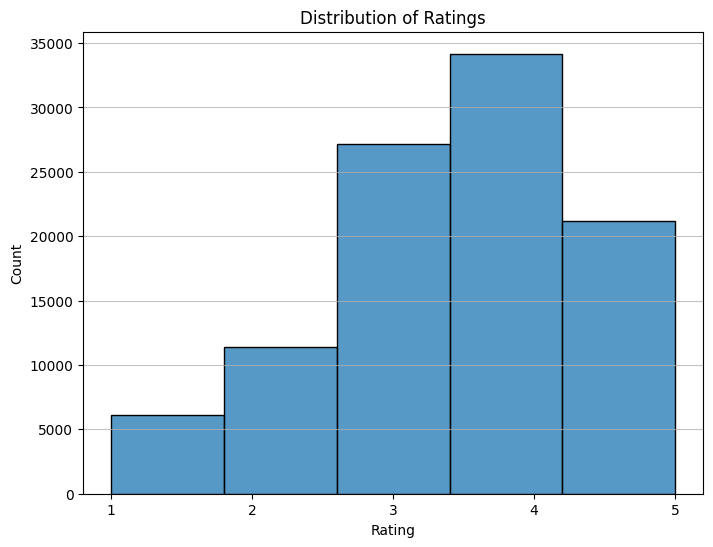
\includegraphics[width=0.7\textwidth]{rating.png}
\end{figure}

Figure \ref{fig:rating-dist} shows how the acquired dataset contain the distribution of discrete user ratings on a 1 to 5 scale. The vertical bar graph describes how many users has a rating of 1, 2, 3, 4, and 5 respectively as seen on the horizontal axis.

\begin{figure}[H]
	\centering
	\caption{Average ratings per users}
	\label{fig:avg-rating-user}
	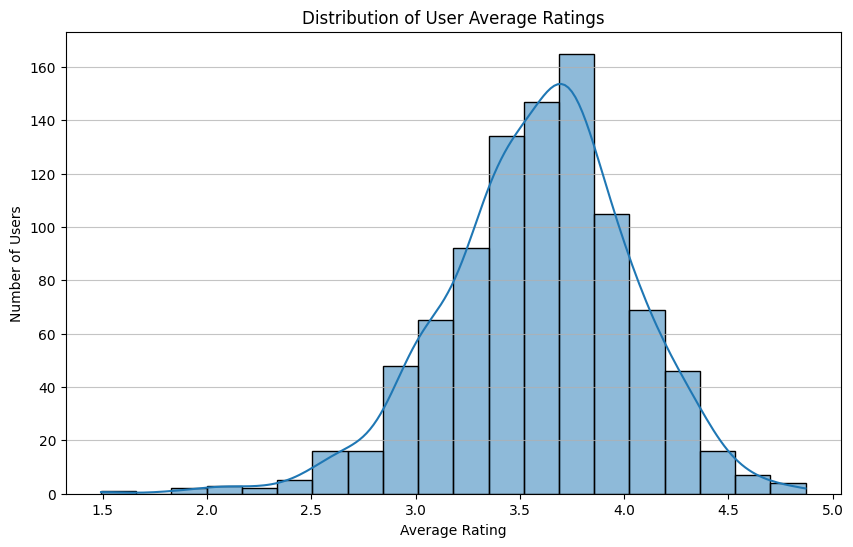
\includegraphics[width=0.7\textwidth]{dist-avg.png}
\end{figure}

Figure \ref{fig:avg-rating-user} shows the average ratings made by all the users. More specifically, the bar graphs in the figure describes the rating behavior of many users on a continuous scale rather than the discrete nature described in Figure 2. Figure 3 most noticeably shows high density of users in the positive end of the scale. This implies that majority of users rates most of their rated items high.

\begin{figure}[H]
	\centering
	\caption{Distribution of User ratings}
	\label{fig:dist-rating}
	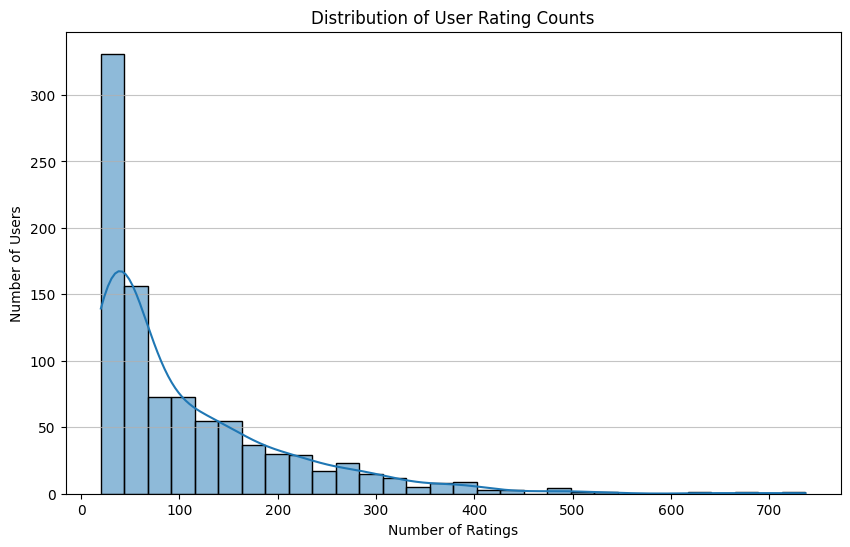
\includegraphics[width=0.7\textwidth]{dist-rating.png}
\end{figure}

Figure \ref{fig:dist-rating} shows the number of ratings that users have made. While the previous two figures show a positively favorable ratings. Figure 4 shows how much of the users rated how many items, which is, as can be seen in the graph, often fall in the range less than 100 but always greater than 0. This implies that while majority of the users has average ratings greater than 3.5, the amount of items they rated are low in comparison.

\section{Experimental Setup for ALS Solver Comparison}

A train-test split was done on the observed ratings, with 80\% of the data used for training and 20\% reserved for testing. The ALS algorithm was implemented with a fixed set of hyperparameters across all solver runs to ensure a fair comparison. The following hyperparameters were used:
\begin{itemize}
		\item Latent dimension \( K = 10 \),
		\item Regularization parameter \( \lambda = 10.0 \),
		\item Training epochs (iterations): 30.
\end{itemize}

These values were chosen to provide a reasonable balance between model complexity and computational feasibility for the benchmark dataset. The same random seed was used for all runs to ensure that the initial latent factor matrices \( U \) and \( V \) were identical across solvers, isolating the effect of the solver choice on performance.

\subsection{System of Linear Equation Solver Implementation}
To ensure a fair comparison, all solvers were implemented in Python and no high-level library functions that abstract away the underlying algorithm were used. This allows for a direct comparison of the computational efficiency and numerical stability of each method in the context of the ALS update step. The solver includes matrix inverse method, Gaussian elimination with Partial pivoting, LU decomposition, QR decomposition, and Cholesky decomposition.

\noindent Each run logs per-epoch quantities for analysis and comparison:
\begin{itemize}
    \item training RMSE,
    \item test RMSE,
    \item elapsed time,
    \item average residual norm $\|Ax-b\|$,
    \item condition number of ALS subproblem matrices.
\end{itemize}

With these metrics, the evaluation not only includes final recommendation quality but also the convergence behavior, computational efficiency, and numerical stability of each solver choice within the ALS framework.

\vspace{4em}

\chapter*{Analysis and Results}

The results of the ALS solver comparison are presented in this section, focusing on the three main evaluation criteria: computational efficiency, numerical stability, and recommendation quality. The analysis includes a discussion of the observed trends and their implications for selecting solvers in practical recommender system implementations.

\section{Alternating Least Squares Convergence}

All solvers showed similar convergence patterns in terms of training and test RMSE over the 30 epochs. The final RMSE values on the test set were effectively identical across solvers, indicating that the choice of linear system solver did not materially affect the quality of the recommendations generated by ALS on this dataset. This suggests that, for well-implemented solvers, the numerical solution to the ALS subproblems is sufficiently accurate to yield comparable model performance.

\begin{table}[h]
	\centering
	\caption{ALS training metrics across epochs}
	\label{tab:training}
	\begin{tabularx}{\linewidth}{XXXXX}
		\toprule
		\textbf{Epoch} & \textbf{Train RMSE} & \textbf{Test RMSE} & \textbf{Loss} & \textbf{$\kappa$(A)} \\
		\midrule
		5 & 0.8533 & 1.0046 & 138{,}674.65 & 18.87 \\
		10 & 0.8166 & 0.9767 & 129{,}916.52 & 15.51 \\
		15 & 0.8096 & 0.9716 & 128{,}839.00 & 15.14 \\
		20 & 0.8073 & 0.9700 & 128{,}623.42 & 15.09 \\
		25 & 0.8065 & 0.9694 & 128{,}569.10 & 15.10 \\
		30 & 0.8061 & 0.9691 & 128{,}549.98 & 15.10 \\
		\bottomrule
	\end{tabularx}
\end{table}

Table \ref{tab:training} shows the training and test RMSE values across epochs, along with the loss and condition number of the ALS subproblem matrices. The RMSE values decrease steadily, indicating that the model is learning effectively, while the condition number remains relatively stable, suggesting that the numerical properties of the subproblems do not degrade significantly over iterations. 

\begin{figure}[H]
	\centering
	\caption{RMSE Progression over Epochs}
	\label{fig:rmse-epochs}
	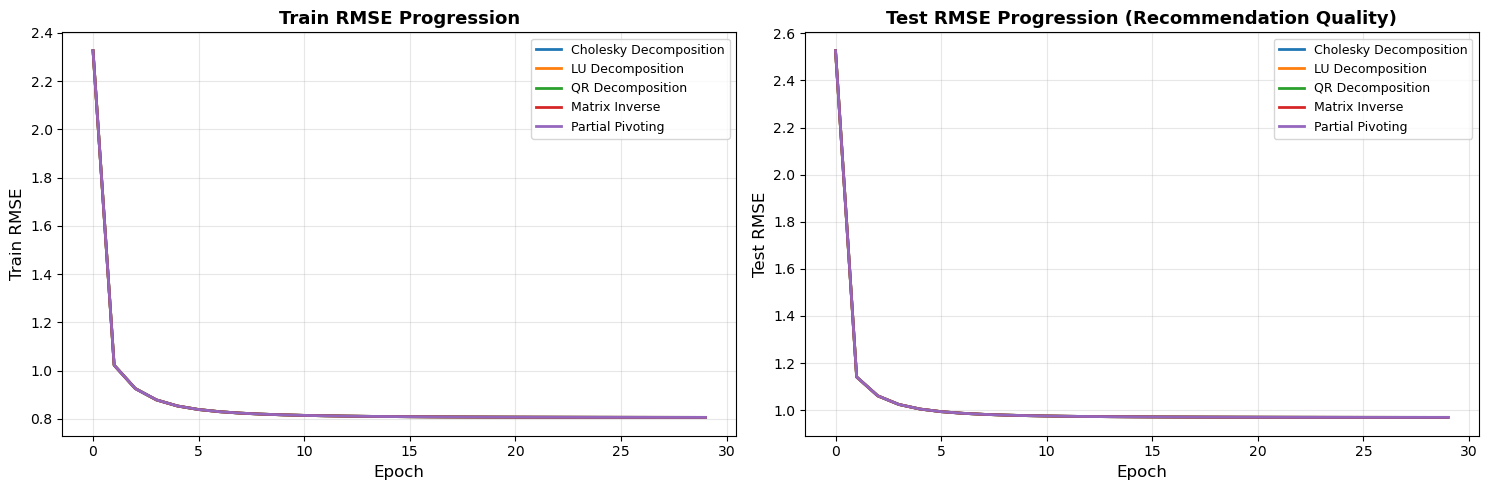
\includegraphics[width=\linewidth]{progression.png}
\end{figure}

Figure \ref{fig:rmse-epochs} visually confirms the convergence behavior, showing that all solvers follow the same trajectory in terms of RMSE reduction, reinforcing the conclusion that solver choice does not impact recommendation quality on this dataset. Further, the progression of both training and test RMSE suggests that the model is not overfitting, as the gap between them remains small and stable across epochs.

\subsection{Runtime and Stability}

Even though recommendation quality was similar across solvers, their runtime and stability differed.

\subsubsection{Runtime Comparison}

\begin{figure}[H]
	\centering
	\caption{Solver Runtime}
	\label{fig:runtime}
	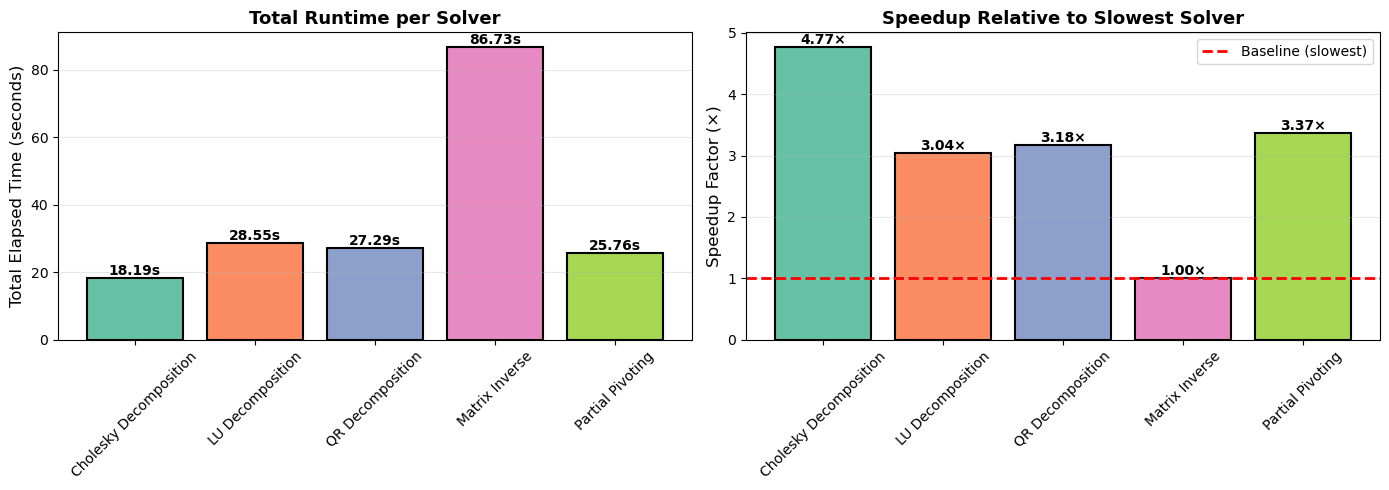
\includegraphics[width=\linewidth]{runtime.png}
\end{figure}

Figure \ref{fig:runtime} shows the runtime for each solver. Cholesky decomposition was the fastest this because it exploits the symmetric positive definite (SPD) structure of the ALS subproblems, while explicit matrix inversion was the slowest due to its computational inefficiency and numerical instability.
LU decomposition, QR decomposition, and Partial pivoting shows almost similar runtime and 3 times faster the matrix inverse method.

\subsubsection{Solver Stability}

\begin{figure}[H]
	\centering
	\caption{Residual Norm Progression}
	\label{fig:resid}
	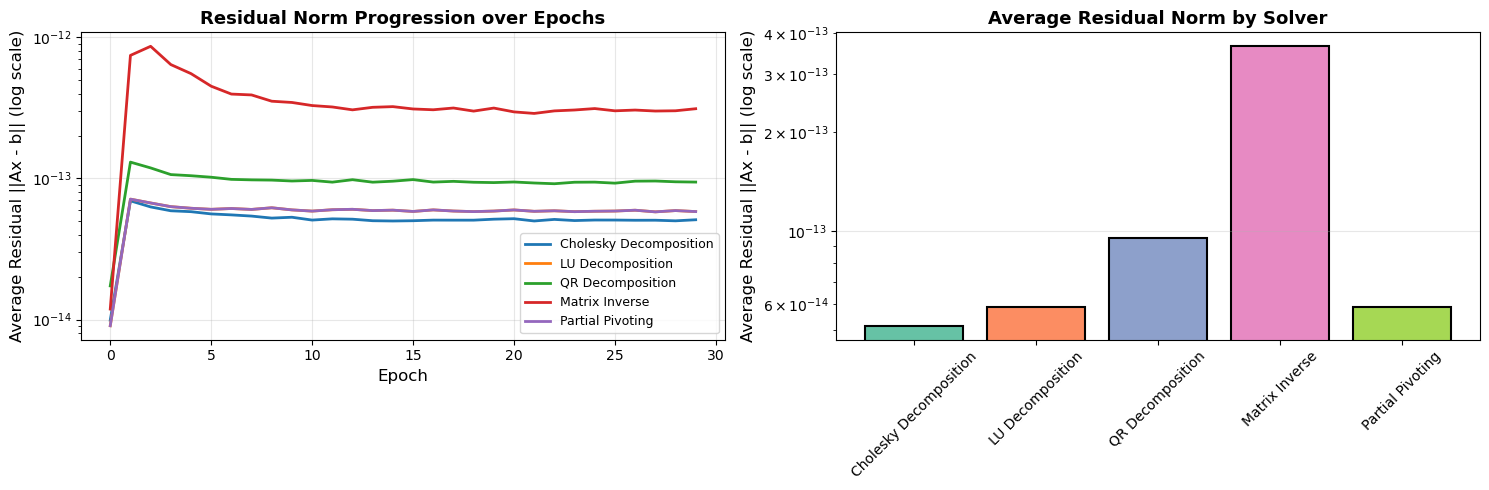
\includegraphics[width=\linewidth]{residual.png}
\end{figure}

Figure \ref{fig:resid} shows the average residual norm $\|Ax-b\|$ for each solver across epochs. The residual norms were lowest for Cholesky decomposition, this is again due to the SPD structure of the ALS subproblems, which allows it to achieve more accurate solutions. The residual progression also shown consistent for each epoch, indicating that the numerical stability of the solvers did not degrade over time.
Explicit matrix inversion had the highest residual norms, reflecting its lower numerical stability. The other solvers had intermediate residual norms, with LU and  partial pivoting achieve a similar level of stability, this is due to the fact the both solvers are based on Gaussian elimination. QR decomposition had slightly higher residual norms than Cholesky, which is expected since it does not exploit the SPD structure as effectively.

\begin{table}[h]
\centering
\caption{Solver Comparison Summary}
\label{tab:solver-comparison}
\begin{tabularx}{\linewidth}{XXXXX}
\toprule
\textbf{Solver} & \textbf{Train RMSE} & \textbf{Test RMSE} & \textbf{Elapsed Time (s)} & \textbf{Avg Residual $\|Ax-b\|$}\\
\midrule
Cholesky Decomposition & 0.806108 & 0.969133 & 18.1859 & $5.15 \times 10^{-14}$  \\
LU Decomposition       & 0.806108 & 0.969133 & 28.5464 & $5.85 \times 10^{-14}$  \\
QR Decomposition       & 0.806108 & 0.969133 & 27.2921 & $9.55 \times 10^{-14}$  \\
Matrix Inverse         & 0.806108 & 0.969133 & 86.7331 & $3.64 \times 10^{-13}$  \\
Partial Pivoting       & 0.806108 & 0.969133 & 25.7574 & $5.85 \times 10^{-14}$  \\
\bottomrule
\end{tabularx}
\end{table}

Table \ref{tab:solver-comparison} summarizes the key metrics for each solver, confirming that while all solvers achieved the same RMSE values, their runtime and numerical stability varied significantly. Cholesky decomposition stands out as the best choice for this problem due to its combination of speed and stability, while explicit matrix inversion is clearly the least favorable option.

\vspace{4em}

\chapter*{Conclusion}
This work evaluated five linear system solvers within ALS for collaborative filtering and showed that, on MovieLens 100K with fixed hyperparameters, recommendation quality is essentially invariant to solver choice. The principal differentiator is computational efficiency, while numerical stability differences are better captured by residual norms than by condition number alone.

The study also established a data-informed context through exploratory analysis, confirming that the rating matrix structure is compatible with ALS modeling and that mild filtering can reduce outlier influence without changing central behavior. Integrating EDA with solver benchmarking provides a clearer basis for engineering decisions than model-metric comparison alone.

For well-conditioned ALS subproblems, practitioners should prioritize fast and stable factorization-based solvers, particularly Cholesky when symmetric positive definite structure is present. For more difficult or ill-conditioned regimes, numerical robustness should be weighted more heavily than raw speed, with residual diagnostics monitored throughout training.

Future work may extend this comparison to larger datasets, different latent dimensions and regularization strengths, and iterative solvers to study scalability and trade-offs in distributed or production-scale recommender systems.
\newpage
% \printbibliography[heading=bibintoc,title={REFERENCES}]

\printbibliography[title={REFERENCES}]
\markboth{}{}
\clearpage
\appendix
\thispagestyle{plain}
\vspace*{\fill}
\begin{center}
		\Huge\textbf{Appendix}
\end{center}
\vspace*{\fill}
\clearpage

\newpage

% \newgeometry{margin=0.75in}
\lstset{
    frame=none,
    aboveskip=2pt,
    belowskip=2pt,
    basicstyle=\ttfamily\footnotesize,
    breaklines=true
}

\chapter*{Appendix: Code Snippets}
\addcontentsline{toc}{chapter}{Appendix: Code Snippets}

\subsection{Alternating Least Squares Engine (als.py)}
\begin{lstlisting}[language=Python, caption={ALS Engine Implementation}]
import numpy as np
import time
from dataclasses import dataclass, field
from typing import List, Callable

# Convergence Tracker
@dataclass
class ALSLog:
  solver_name   : str
  train_rmse    : List[float] = field(default_factory=list)
  test_rmse     : List[float] = field(default_factory=list)
  train_loss    : List[float] = field(default_factory=list)
  residual_norm : List[float] = field(default_factory=list)
  cond_number   : List[float] = field(default_factory=list)
  elapsed_time  : List[float] = field(default_factory=list)

  def rmse_delta(self):
    tr = self.train_rmse
    return [abs(tr[i] - tr[i-1]) for i in range(1, len(tr))]

  def epoch_to_convergence(self, eps=1e-4):
    for i, d in enumerate(self.rmse_delta()):
      if d < eps: return i + 2
    return None

# Metric Helpers
def _rmse(R_true, U, V):
  mask = R_true > 0
  pred = (U @ V.T)[mask]
  return float(np.sqrt(np.mean((pred - R_true[mask]) ** 2)))

def _reg_loss(R, U, V, lam):
  mask = R > 0
  pred = (U @ V.T)[mask]
  return float(np.sum((pred - R[mask]) ** 2) 
               + lam * (np.sum(U ** 2) + np.sum(V ** 2)))

def _safe_cond(A):
  try:
    return float(np.linalg.cond(A))
  except np.linalg.LinAlgError:
    return float('inf')

# ALS Engine
def run_als(R_train, R_test, solver_fn, solver_name, k=10, lam=0.1, n_epochs=50, seed=42, verbose=True):
  log = ALSLog(solver_name=solver_name)
  np.random.seed(seed)
  n_users, n_items = R_train.shape
  lam_I = lam * np.eye(k)
  U = np.random.normal(0, 0.1, (n_users, k))
  V = np.random.normal(0, 0.1, (n_items, k))
  user_items = [np.where(R_train[u] > 0)[0] for u in range(n_users)]
  item_users = [np.where(R_train[:, i] > 0)[0] for i in range(n_items)]
  t0 = time.time()

  for epoch in range(n_epochs):
    ep_res, ep_cond = [], []
    for u in range(n_users):
      rated = user_items[u]
      if len(rated) == 0: continue
      V_Iu, r_u = V[rated], R_train[u, rated]
      A, b = V_Iu.T @ V_Iu + lam_I, V_Iu.T @ r_u
      x, res = solver_fn(A, b)
      U[u] = x
      ep_res.append(res); ep_cond.append(_safe_cond(A))

    for i in range(n_items):
      rated = item_users[i]
      if len(rated) == 0: continue
      U_Ii, r_i = U[rated], R_train[rated, i]
      A, b = U_Ii.T @ U_Ii + lam_I, U_Ii.T @ r_i
      x, res = solver_fn(A, b)
      V[i] = x
      ep_res.append(res); ep_cond.append(_safe_cond(A))

    log.train_rmse.append(_rmse(R_train, U, V))
    log.test_rmse.append(_rmse(R_test, U, V))
    log.train_loss.append(_reg_loss(R_train, U, V, lam))
    log.residual_norm.append(float(np.mean(ep_res)))
    log.cond_number.append(float(np.mean(ep_cond)))
    log.elapsed_time.append(time.time() - t0)
  return log
\end{lstlisting}

\subsection{Matrix Inverse Solver}
\begin{lstlisting}[language=Python, caption={Matrix Inverse Implementation}]
import numpy as np

def matrix_inverse(A, b):
    k = len(b)
    aug = np.zeros((k, 2 * k))
    for i in range(k):
        for j in range(k): aug[i, j] = float(A[i, j])
        aug[i, k + i] = 1.0

    for col in range(k):
        max_row = col + np.argmax(np.abs(aug[col:, col]))
        aug[[col, max_row]] = aug[[max_row, col]]
        pivot = aug[col, col]
        aug[col] /= pivot
        for row in range(k):
            if row == col: continue
            aug[row] -= aug[row, col] * aug[col]

    A_inv = aug[:, k:]
    x = A_inv @ b
    res = float(np.sqrt(np.sum((A @ x - b) ** 2)))
    return x, res
\end{lstlisting}

\subsection{Partial Pivoting Solver}
\begin{lstlisting}[language=Python, caption={Gaussian Elimination Implementation}]
import numpy as np

def partial_pivoting(A, b):
    k = len(b)
    M = np.column_stack((A.astype(float), b.astype(float)))
    for col in range(k):
        max_row = col + np.argmax(np.abs(M[col:, col]))
        M[[col, max_row]] = M[[max_row, col]]
        for row in range(col + 1, k):
            factor = M[row, col] / M[col, col]
            M[row, col:] -= factor * M[col, col:]

    x = np.zeros(k)
    for i in range(k - 1, -1, -1):
        x[i] = (M[i, k] - np.dot(M[i, i+1:k], x[i+1:k])) / M[i, i]
    res = float(np.sqrt(np.sum((A @ x - b) ** 2)))
    return x, res
\end{lstlisting}

\subsection{LU Decomposition Solver}
\begin{lstlisting}[language=Python, caption={LU Decomposition Implementation}]
import numpy as np

def lu_decomposition(A, b):
    k = len(b)
    L, U, P = np.eye(k), A.astype(float).copy(), np.eye(k)
    for col in range(k):
        max_row = col + np.argmax(np.abs(U[col:, col]))
        U[[col, max_row]], P[[col, max_row]] = U[[max_row, col]], P[[max_row, col]]
        L[[col, max_row], :col] = L[[max_row, col], :col]
        for row in range(col + 1, k):
            L[row, col] = U[row, col] / U[col, col]
            U[row, col:] -= L[row, col] * U[col, col:]

    pb = P @ b
    y = np.zeros(k)
    for i in range(k): y[i] = pb[i] - np.dot(L[i, :i], y[:i])
    x = np.zeros(k)
    for i in range(k - 1, -1, -1): x[i] = (y[i] - np.dot(U[i, i+1:], x[i+1:])) / U[i, i]
    res = float(np.sqrt(np.sum((A @ x - b) ** 2)))
    return x, res
\end{lstlisting}

\subsection{QR Decomposition Solver}
\begin{lstlisting}[language=Python, caption={QR Decomposition Implementation}]
import numpy as np

def qr_decomposition(A, b):
    k = len(b)
    R, b_hat = A.astype(float).copy(), b.astype(float).copy()
    for j in range(k):
        v = R[j:, j].copy()
        v[0] += (1.0 if v[0] >= 0.0 else -1.0) * np.sqrt(np.dot(v, v))
        norm_v = np.sqrt(np.dot(v, v))
        if norm_v == 0: continue
        v /= norm_v
        R[j:, j:] -= 2.0 * np.outer(v, np.dot(v, R[j:, j:]))
        b_hat[j:] -= 2.0 * v * np.dot(v, b_hat[j:])
    x = np.zeros(k)
    for i in range(k - 1, -1, -1): x[i] = (b_hat[i] - np.dot(R[i, i+1:], x[i+1:])) / R[i, i]
    res = float(np.sqrt(np.sum((A @ x - b) ** 2)))
    return x, res
\end{lstlisting}

\subsection{Cholesky Decomposition Solver}
\begin{lstlisting}[language=Python, caption={Cholesky Decomposition Implementation}]
import numpy as np

def cholesky_decomposition(A, b):
    k = len(b)
    L = np.zeros((k, k))
    for j in range(k):
        s = A[j, j] - np.dot(L[j, :j], L[j, :j])
        L[j, j] = np.sqrt(max(s, 0))
        for i in range(j + 1, k):
            L[i, j] = (A[i, j] - np.dot(L[i, :j], L[j, :j])) / L[j, j]
    y = np.zeros(k)
    for i in range(k): y[i] = (b[i] - np.dot(L[i, :i], y[:i])) / L[i, i]
    x = np.zeros(k)
    for i in range(k - 1, -1, -1): x[i] = (y[i] - np.dot(L[i+1:, i], x[i+1:])) / L[i, i]
    res = float(np.sqrt(np.sum((A @ x - b) ** 2)))
    return x, res
\end{lstlisting}

\restoregeometry


\end{document}
